\section{Identifying Secondary Metabolite Biosynthetic Gene Clusters}
\label{section:secondary-metabolites}

Due to time constraints, only a cursory analysis of secondary metabolite
biosynthetic gene clusters was performed on the Tsth20 assembly using the software \textit{antiSMASH}. Tsth20 was selected for this analysis as it is the most contiguous assembly produced in this study, and it is of particular interest due to its observed interactions with plants.

From the Braker2 gene predictions, antiSMASH identified 35 candidate secondary metabolite biosynthetic gene clusters in the Tsth20 assembly, while GeneMark identified 58 clusters. These clusters varied in length from 30kb to 130kb. The RefSeq annotation for Tsth20 was not available for analysis with antiSMASH. The types of secondary metabolite clusters identified included non-ribosomal peptide synthetases (NRPS), polyketide synthases (PKS), and terpenes. Example clusters identified by antiSMASH from Braker2 and GeneMark gene predictions from contig ctg000020 are shown in Figure~\ref{fig:antismash-clusters}. From Figure~\ref{fig:antismash-clusters}, we can see that both gene prediction methods identified similar clusters, although GeneMark identified a greater number of clusters overall. This may be a result of Braker2 being trained on \textit{T. reesei} gene models, which could lead to a bias in predictions towards genes similar to those in \textit{T. reesei} resulting in missed or incorrectly predicted clusters. The trend of GeneMark marks gene predictions being more sensitive than Braker2 predictions continues for the other contigs in Tsth20, except in the case of ctg000000, in which antiSMASH identified no clusters from Braker2 predictions.

\begin{figure}
  \centering
  \begin{subfigure}{0.90\textwidth}
    \centering
    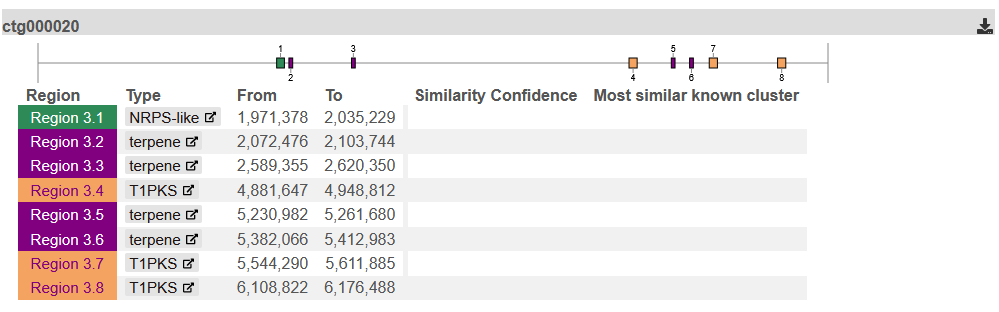
\includegraphics[width=\textwidth]{figures/braker-antismash-tsth20.png}
    \caption{Clusters from Braker2 gene predictions}
  \end{subfigure}
  \begin{subfigure}{0.9\textwidth}
    \centering
    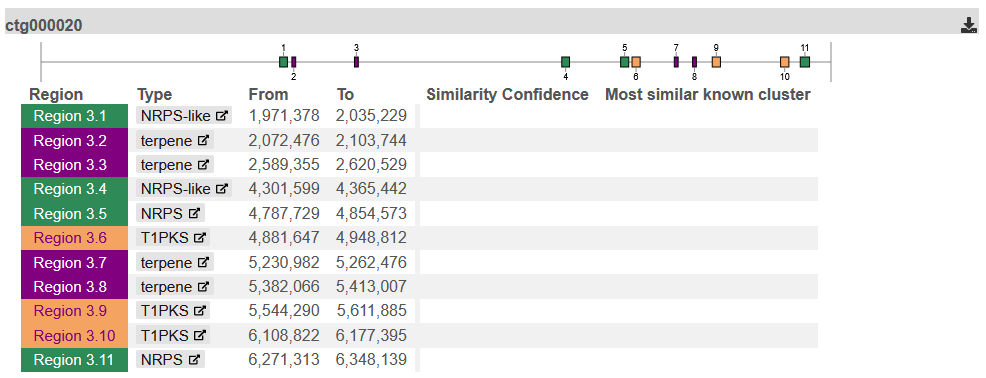
\includegraphics[width=\textwidth]{figures/genemark-antismash-tsth20.png}
    \caption{Clusters from GeneMark gene predictions}
  \end{subfigure}
  \caption[Example Secondary Metabolite Gene Clusters Identified by antiSMASH]{Example secondary metabolite gene clusters identified by antiSMASH from Braker2 (top) and GeneMark (bottom) gene predictions from contig ctg000020 in the Tsth20 assembly.}\label{fig:antismash-clusters}
\end{figure}

While these results are promising, a more thorough analysis of secondary metabolite gene clusters across all assemblies using multiple gene prediction methods would be necessary to draw any meaningful conclusions about the secondary metabolite potential of these \textit{Trichoderma} strains. Future work could also involve cross-referencing identified clusters with known secondary metabolites and functional annotations to better understand their roles and biosynthetic pathways.